% !TeX program = lualatex
% ================================================================
% Polish Tier 3 Vocabulary Version of ProbabilityStarters
%
% Generated by the server using the following settings:
%
%   language            Polish (pol)
%   text direction      left to right
%   font                Noto Serif
%   fallback font       Noto Serif
%   built from          latex/starters/targeted/KS3/probability/probabilityStarters.tex
%   vocabulary key      latex/starters/targeted/KS3/probability/probabilityStarters/L2/pol/probabilityStarters_polishKey.tex
%   tier 3 vocabulary   green   RGB 0 128 0
%   English text        black   RGB 0 0 0
%   Polish text         purple  RGB 112 48 160
%   layout macros       version 3
%
% Please don't edit any information in this comment block - the server
% compares it against the current settings and rebuilds this file when
% they differ, so changes here would be overwritten. However, feel free
% to make updates to the LaTeX below if you want to edit it.
% ================================================================

\documentclass{beamer}
% ================================================================
% Copied from the English sheet this was translated from, so that
% anything it sets up for itself still works here
% ================================================================
\usepackage{tikz}
\usetikzlibrary{calc}
\usetikzlibrary{decorations.pathreplacing}
\usepackage{multicol}
\usepackage{amsmath}

\setbeamertemplate{navigation symbols}{}
\setbeamersize{text margin left=0.4cm, text margin right=0.4cm}
\setlength{\multicolsep}{4pt}
% wide enough that an enumerate label in the second column of a multicols still has a
% clear word space in front of it, whatever the first column's line does
\setlength{\columnsep}{18pt}
\renewcommand{\arraystretch}{0.92}

% ================================================================
% Answer-overlay helpers
% ================================================================
\newcommand{\ablank}[1]{%
  \alt<2>{\textcolor{red}{#1}}{\underline{\phantom{#1}}}%
}
\newcommand{\ashow}[1]{\uncover<2->{\textcolor{red}{\small #1}}}
\newcommand{\ashowq}[1]{\alt<2->{\textcolor{red}{\small #1}}{?}}

% Answers drawn straight on to a TikZ diagram, revealed on overlay 2 like \ashow.
% Space is reserved on overlay 1, so the diagram does not move between slides.
\usetikzlibrary{overlay-beamer-styles}
\tikzset{
  ans/.style     = {red, thick, visible on=<2->},
  ansfill/.style = {red!15, visible on=<2->},
  anslab/.style  = {red, font=\tiny, visible on=<2->},
}

% Used by the worked solutions rather than by this deck, so that each worked
% solution is first a question with room to write in and then the answer.
\newlength{\aworkpad}
\setlength{\aworkpad}{8mm}
\newcommand{\awork}[1]{%
  \par\vspace{\aworkpad}%
  \uncover<2->{#1}%
  \par\vspace{\aworkpad}%
}

% A gap inside a TikZ node: a question mark on the first overlay and the answer in
% red on the second. Unlike \ashowq this leaves the node's own font alone, so a gap
% in a frequency tree or a Venn diagram is the same size as the numbers beside it.
\newcommand{\dgap}[1]{\alt<2->{\textcolor{red}{#1}}{?}}

% Every question list on these slides is tight, so that the diagram column and
% the question column both finish inside the slide.
\newcommand{\tightlist}{%
  \setlength{\itemsep}{0pt}\setlength{\parskip}{0pt}\setlength{\topsep}{0pt}%
}

% ================================================================
% The pictures these starters are built from.
%
% Every picture is drawn at scale 1, with its coordinates given in centimetres,
% because a TikZ scale factor shrinks the coordinates but not the text or the node
% sizes, which is what makes labels collide in a narrow column.
% ================================================================

% The outline of an open cloth bag, \bag{width}{height}, drawn from the origin.
\newcommand{\bag}[2]{%
  \draw[thick, rounded corners=3pt, fill=brown!12]
    (0,0) -- (0,#2) -- (-0.22,{#2+0.5}) -- ({#1+0.22},{#2+0.5})
       -- (#1,#2) -- (#1,0) -- cycle;}

% One counter, \ctr{x}{y}{colour}{letter}. The letter is printed on the counter so
% that the colours can still be told apart on a projector or on a photocopy.
\newcommand{\ctr}[4]{%
  \draw[fill=#3, draw=black!55, line width=0.4pt] (#1,#2) circle (0.28);
  \node[font=\tiny] at (#1,#2) {#4};}

% One chocolate in a box, \choc{x}{y}{colour}{letter}.
\newcommand{\choc}[4]{%
  \draw[fill=#3, draw=black!60, line width=0.35pt, rounded corners=1.5pt]
    ({#1-0.28},{#2-0.26}) rectangle ({#1+0.28},{#2+0.26});
  \node[font=\tiny] at (#1,#2) {#4};}

% The items on a lunch menu: \sarnie{x}{y}{letter} and \drink{x}{y}{letter}.
\newcommand{\sarnie}[3]{%
  \draw[fill=orange!25, draw=black!60, line width=0.4pt]
    ({#1-0.34},{#2-0.26}) -- ({#1+0.34},{#2-0.26}) -- (#1,{#2+0.3}) -- cycle;
  \node[font=\tiny] at (#1,{#2-0.09}) {#3};}
\newcommand{\drink}[3]{%
  \draw[fill=blue!18, draw=black!60, line width=0.4pt]
    ({#1-0.19},{#2-0.3}) -- ({#1+0.19},{#2-0.3}) -- ({#1+0.27},{#2+0.3})
    -- ({#1-0.27},{#2+0.3}) -- cycle;
  \node[font=\tiny] at (#1,#2) {#3};}

\tikzset{
  % the circles of a frequency tree, all one size so that a gap does not move them
  ftnode/.style  = {draw, circle, minimum size=0.62cm, inner sep=0pt, font=\scriptsize},
  % fill=white so that a branch label masks the branch it sits on
  ftlab/.style   = {font=\tiny, inner sep=1.5pt, fill=white},
  ftarrow/.style = {-, thick},
  % the two sets of a Venn diagram and the numbers written inside its regions
  vset/.style = {thick},
  vnum/.style = {font=\small},
  vlab/.style = {font=\scriptsize},
}

\title{Probability: Starters}
\author{}
\date{}

% Characters this language's font has not got are borrowed from another,
% rather than being silently dropped - see docs/translated-sheet-latex.md
\directlua{%
  if luaotfload and luaotfload.add_fallback then
    luaotfload.add_fallback("eallatinfallback",
      { "Noto Serif:mode=harf;" })
  else
    tex.error("this luaotfload is too old to register a fallback font")
  end
}
\usepackage[english]{babel}
\babelprovide[import]{polish}
\babelfont[polish]{rm}[Renderer=Harfbuzz, BoldFont={Noto Serif}, ItalicFont={Noto Serif}, BoldItalicFont={Noto Serif}, RawFeature={fallback=eallatinfallback}]{Noto Serif}
\babelfont[polish]{sf}[Renderer=Harfbuzz, BoldFont={Noto Serif}, ItalicFont={Noto Serif}, BoldItalicFont={Noto Serif}, RawFeature={fallback=eallatinfallback}]{Noto Serif}
\newcommand{\ealtext}[1]{\foreignlanguage{polish}{#1}}
\newcommand{\ealtextblock}[1]{{\raggedright\foreignlanguage{polish}{#1}\par}}
% ================================================================
% EAL layout helpers
% ================================================================
\usepackage{xcolor}

\definecolor{ealkeycolour}{RGB}{0,128,0}
\definecolor{ealenglish}{RGB}{0,0,0}
\definecolor{ealtwocolour}{RGB}{112,48,160}

\newsavebox{\ealboxen}
\newsavebox{\ealboxtr}
\newlength{\ealglosswd}
\newlength{\ealglossraise}
\setlength{\ealglossraise}{1.15em}

% a tier 3 word, in English and in translation alike
\newcommand{\ealkey}[1]{\textcolor{ealkeycolour}{#1}}
\newcommand{\ealkeytr}[1]{\textcolor{ealkeycolour}{\ealtext{#1}}}

% One translated word above one English word. Built from kernel
% primitives, never a tabular, which would break wherever the sheet
% loads array, booktabs or tabularx. The box is as wide as the wider of
% the two, so a long translation pushes its neighbours aside instead of
% overlapping them, and it claims its full height so a table row or a
% TikZ node makes room for it.
\newcommand{\ealgloss}[2]{%
  \sbox{\ealboxen}{\ealkey{#1}}%
  \sbox{\ealboxtr}{\small\textcolor{ealtwocolour}{\ealtext{#2}}}%
  \setlength{\ealglosswd}{\wd\ealboxen}%
  \ifdim\wd\ealboxtr>\ealglosswd\setlength{\ealglosswd}{\wd\ealboxtr}\fi
  \leavevmode
  \makebox[\ealglosswd][c]{%
    \makebox[0pt][c]{\usebox{\ealboxen}}%
    \makebox[0pt][c]{\raisebox{\ealglossraise}{\usebox{\ealboxtr}}}%
  }%
}

% opens up line spacing around a block of glosses, so the raised
% translations sit clear of the line above
\newenvironment{ealglossed}{\par\linespread{2.1}\selectfont\ignorespaces}{\par}

% a whole translated sentence above its English counterpart. block level,
% so it does not belong inside a tabular cell
\newcommand{\ealpara}[2]{%
  \par\addvspace{0.5\baselineskip}%
  {\color{ealtwocolour}\ealtextblock{#1}}%
  \penalty200
  {\color{ealenglish}#2\par}%
  \addvspace{0.5\baselineskip}%
}

\begin{document}

\frame{\titlepage}

%------------------------------------------------------------------
% STARTER 1: The probability scale and the words we describe it with
%------------------------------------------------------------------
\begin{frame}[t,allowframebreaks]{Starter}
\begin{columns}[T]

\column{0.42\textwidth}
\begin{center}
\vspace{-0.8em}
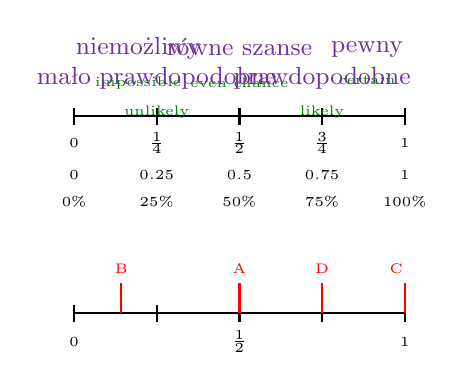
\begin{tikzpicture}[every node/.style={font=\tiny}]

% ---- The probability scale, with the words and the numbers on it ----
\draw[thick] (0,0) -- (4.2,0);
\foreach \x in {0,1.05,2.1,3.15,4.2} \draw[thick] (\x,-0.11) -- (\x,0.11);
% the words sit at two heights, so that they do not run into each other
\node[anchor=west] at (-0.10,0.68) {\ealgloss{impossible}{niemożliwy}};
\node at (2.1,0.68) {\ealgloss{even chance}{równe szanse}};
\node[anchor=east] at (4.30,0.68) {\ealgloss{certain}{pewny}};
\node at (1.05,0.30) {\ealgloss{unlikely}{mało prawdopodobne}};
\node at (3.15,0.30) {\ealgloss{likely}{prawdopodobne}};
% the same probabilities written as a fraction, a decimal and a percentage
\foreach \x/\f/\d/\p in {%
   0/$0$/$0$/$0\%$,
   1.05/$\tfrac{1}{4}$/$0.25$/$25\%$,
   2.1/$\tfrac{1}{2}$/$0.5$/$50\%$,
   3.15/$\tfrac{3}{4}$/$0.75$/$75\%$,
   4.2/$1$/$1$/$100\%$}{
  \node at (\x,-0.34) {\f};
  \node at (\x,-0.74) {\d};
  \node at (\x,-1.08) {\p};
}

% ---- An empty scale, for marking the four events on ----
\draw[thick] (0,-2.5) -- (4.2,-2.5);
\foreach \x in {0,1.05,2.1,3.15,4.2} \draw[thick] (\x,-2.61) -- (\x,-2.39);
\node at (0,-2.86) {$0$};
\node at (2.1,-2.86) {$\tfrac{1}{2}$};
\node at (4.2,-2.86) {$1$};

% the answers to question 4, marked on the empty scale
\draw[ans] (0.60,-2.50) -- (0.60,-2.12);
\node[anslab] at (0.60,-1.94) {B};
\draw[ans] (2.1,-2.50) -- (2.1,-2.12);
\node[anslab] at (2.1,-1.94) {A};
\draw[ans] (3.15,-2.50) -- (3.15,-2.12);
\node[anslab] at (3.15,-1.94) {D};
\draw[ans] (4.2,-2.50) -- (4.2,-2.12);
\node[anslab, anchor=east] at (4.30,-1.94) {C};

\end{tikzpicture}
\end{center}
\vspace{0.2em}
\begin{ealglossed}
{\tiny\raggedright
\textbf{A} \ a \ealgloss{fair}{uczciwa} coin lands on heads\\
\textbf{B} \ a day chosen at \ealgloss{random}{losowo} is a Saturday\\
\textbf{C} \ an ordinary dice is rolled and shows a number less than $7$\\
\textbf{D} \ a counter taken from a bag of $3$ red and $1$ blue counters is red\par}
\end{ealglossed}

\column{0.58\textwidth}
\vspace{-1.8em}
\footnotesize
\begin{ealglossed}
\begin{enumerate}\tightlist
\begin{multicols}{2}
  \item Write $0.25$ as a \ealgloss{fraction}{ułamek} in its \ealgloss{simplest form}{najprostsza postać}.
        \ashow{$\tfrac{1}{4}$}
  \columnbreak
  \item Write $\dfrac{3}{5}$ as a \ealgloss{decimal}{ułamek dziesiętny} and as a \ealgloss{percentage}{procent}.
        \ashow{$0.6=60\%$}
\end{multicols}
\begin{multicols}{2}
  \item Every \ealgloss{probability}{prawdopodobieństwo} is a number from \ablank{$\;0\;$} to \ablank{$\;\;1$}.
  \columnbreak
  \item Mark \ealgloss{events}{zdarzenia} \textbf{A}, \textbf{B}, \textbf{C} and \textbf{D} on the empty \ealgloss{scale}{skalować}.
\end{multicols}
  \item Complete the table.
  \begin{center}
  {\scriptsize\renewcommand{\arraystretch}{1.6}\setlength{\tabcolsep}{5pt}
  \begin{tabular}{l|c}
    Description & \ealgloss{Probability}{prawdopodobieństwo}\\ \hline
    \ealgloss{impossible}{niemożliwy}  & $0$\\
    \ealgloss{unlikely}{mało prawdopodobne}    & between $0$ and \ablank{$0.5$}\\
    \ealgloss{even chance}{równe szanse} & \ablank{$0.5$}\\
    \ealgloss{likely}{prawdopodobne}      & between \ablank{$0.5$} and $1$\\
    \ealgloss{certain}{pewny}     & \ablank{$1$}
  \end{tabular}}
  \end{center}
  \vspace{0.25em}
  \item Write a \ealgloss{probability}{prawdopodobieństwo} that is \ealgloss{unlikely}{mało prawdopodobne} but not \ealgloss{impossible}{niemożliwe}, as a \ealgloss{fraction}{ułamek}, a \ealgloss{decimal}{ułamek dziesiętny}
        and a \ealgloss{percentage}{procent}.
        \ashow{Between $0$ and $0.5$, such as $\tfrac{1}{10}=0.1=10\%$.}
  \item Ravi says ``the \ealgloss{probability}{prawdopodobieństwo} that it rains tomorrow is $1.4$''. Explain why he is wrong.
        \ashow{No \ealgloss{probability}{prawdopodobieństwo} is greater than $1$; a \ealgloss{probability}{prawdopodobieństwo} of $1$ means \ealgloss{certain}{pewne}.}
\end{enumerate}
\end{ealglossed}
\end{columns}
\end{frame}

%------------------------------------------------------------------
% STARTER 2: Probabilities from a bag of counters
%------------------------------------------------------------------
\begin{frame}[t,allowframebreaks]{Starter}
\begin{columns}[T]

\column{0.38\textwidth}
\begin{center}
\vspace{-0.6em}
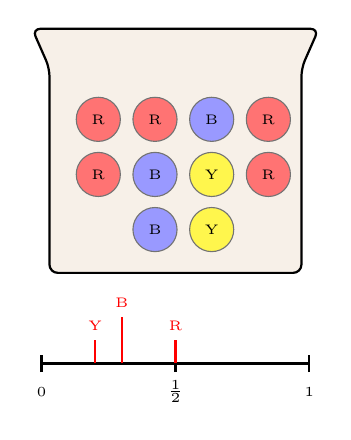
\begin{tikzpicture}[every node/.style={font=\tiny}]

% ---- A bag holding 5 red, 3 blue and 2 yellow counters ----
\bag{3.2}{2.6}
\ctr{0.62}{1.95}{red!55}{R}
\ctr{1.34}{1.95}{red!55}{R}
\ctr{2.06}{1.95}{blue!40}{B}
\ctr{2.78}{1.95}{red!55}{R}
\ctr{0.62}{1.25}{red!55}{R}
\ctr{1.34}{1.25}{blue!40}{B}
\ctr{2.06}{1.25}{yellow!70}{Y}
\ctr{2.78}{1.25}{red!55}{R}
\ctr{1.34}{0.55}{blue!40}{B}
\ctr{2.06}{0.55}{yellow!70}{Y}

% ---- A probability scale to mark the three probabilities on ----
\draw[thick] (-0.1,-1.15) -- (3.3,-1.15);
\foreach \x in {-0.1,1.6,3.3} \draw[thick] (\x,-1.26) -- (\x,-1.04);
\node at (-0.1,-1.51) {$0$};
\node at (1.6,-1.51) {$\tfrac{1}{2}$};
\node at (3.3,-1.51) {$1$};

% the answers to question 7, marked on the scale
\draw[ans] (0.58,-1.15) -- (0.58,-0.85);
\node[anslab] at (0.58,-0.67) {Y};
\draw[ans] (0.92,-1.15) -- (0.92,-0.56);
\node[anslab] at (0.92,-0.38) {B};
\draw[ans] (1.6,-1.15) -- (1.6,-0.85);
\node[anslab] at (1.6,-0.67) {R};

\end{tikzpicture}
\end{center}
\vspace{0.2em}
\begin{ealglossed}
{\scriptsize\raggedright One counter is taken from the bag at \ealgloss{random}{losowo}. The \ealgloss{probability}{prawdopodobieństwo}
that the counter is red is written $P(\text{red})$.\par}
\end{ealglossed}

\column{0.62\textwidth}
\vspace{-1.8em}
\footnotesize
\begin{ealglossed}
\begin{enumerate}\tightlist
\begin{multicols}{2}
  \item Write $\dfrac{1}{2}$ as a \ealgloss{decimal}{ułamek dziesiętny} and as a \ealgloss{percentage}{procent}.
        \ashow{$0.5=50\%$}
  \columnbreak
  \item Write $30\%$ as a \ealgloss{fraction}{ułamek} in its \ealgloss{simplest form}{najprostsza postać}.
        \ashow{$\tfrac{30}{100}=\tfrac{3}{10}$}
\end{multicols}
\begin{multicols}{2}
  \item How many counters are in the bag altogether?
        \ashow{$10$}
  \columnbreak
  \item Write $P(\text{red})$ as a \ealgloss{fraction}{ułamek} in its \ealgloss{simplest form}{najprostsza postać}.
        \ashow{$\tfrac{5}{10}=\tfrac{1}{2}$}
\end{multicols}
\begin{multicols}{2}
  \item Write $P(\text{blue})$ as a \ealgloss{fraction}{ułamek}, a \ealgloss{decimal}{ułamek dziesiętny} and a \ealgloss{percentage}{procent}.
        \ashow{$\tfrac{3}{10}=0.3=30\%$}
  \columnbreak
  \item Mark $P(\text{red})$, $P(\text{blue})$ and $P(\text{yellow})$ on the
        \ealgloss{probability}{prawdopodobieństwo} \ealgloss{scale}{skalować}.
\end{multicols}
\begin{multicols}{2}
  \item Write $P(\text{not red})$ as a \ealgloss{fraction}{ułamek} in its \ealgloss{simplest form}{najprostsza postać}.
        \ashow{$\tfrac{5}{10}=\tfrac{1}{2}$}
  \columnbreak
  \item What does $P(\text{red})+P(\text{blue})+P(\text{yellow})$ come to, and why?
        \ashow{$1$; the counter is \ealgloss{certain}{pewny} to be one of the three colours.}
\end{multicols}
  \item Only red counters are added to the bag, until $P(\text{red})$ is $\tfrac{3}{4}$.
        How many red counters are added?
        \ashow{$10$, giving $15$ red counters out of $20$, and $\tfrac{15}{20}=\tfrac{3}{4}$.}
\end{enumerate}
\end{ealglossed}
\end{columns}
\end{frame}

%------------------------------------------------------------------
% STARTER 3: Comparing probabilities, and expected numbers
%------------------------------------------------------------------
\begin{frame}[t,allowframebreaks]{Starter}
\begin{columns}[T]

\column{0.35\textwidth}
\begin{center}
\vspace{-0.6em}
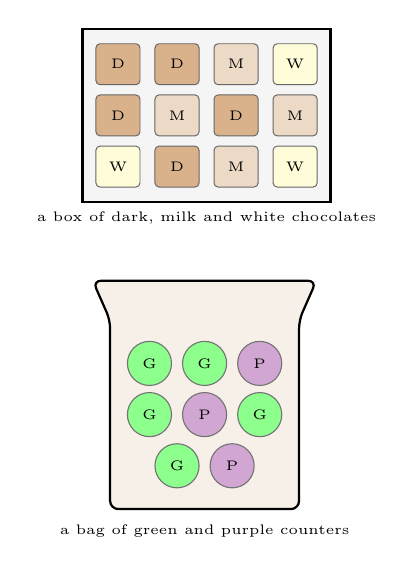
\begin{tikzpicture}[every node/.style={font=\tiny}]

% ---- A box holding 5 dark, 4 milk and 3 white chocolates ----
\draw[thick, fill=gray!8] (0,0) rectangle (3.15,2.2);
\choc{0.45}{1.75}{brown!60}{D}
\choc{1.2}{1.75}{brown!60}{D}
\choc{1.95}{1.75}{brown!30}{M}
\choc{2.7}{1.75}{yellow!15}{W}
\choc{0.45}{1.1}{brown!60}{D}
\choc{1.2}{1.1}{brown!30}{M}
\choc{1.95}{1.1}{brown!60}{D}
\choc{2.7}{1.1}{brown!30}{M}
\choc{0.45}{0.45}{yellow!15}{W}
\choc{1.2}{0.45}{brown!60}{D}
\choc{1.95}{0.45}{brown!30}{M}
\choc{2.7}{0.45}{yellow!15}{W}
\node at (1.575,-0.20) {a box of dark, milk and white chocolates};

% ---- A bag holding 5 green and 3 purple counters ----
\begin{scope}[yshift=-3.9cm, xshift=0.35cm]
\bag{2.4}{2.4}
\ctr{0.5}{1.85}{green!45}{G}
\ctr{1.2}{1.85}{green!45}{G}
\ctr{1.9}{1.85}{violet!35}{P}
\ctr{0.5}{1.2}{green!45}{G}
\ctr{1.2}{1.2}{violet!35}{P}
\ctr{1.9}{1.2}{green!45}{G}
\ctr{0.85}{0.55}{green!45}{G}
\ctr{1.55}{0.55}{violet!35}{P}
\node at (1.2,-0.28) {a bag of green and purple counters};
\end{scope}

\end{tikzpicture}
\end{center}

\column{0.65\textwidth}
\vspace{-1.8em}
\footnotesize
\begin{ealglossed}
\begin{enumerate}\tightlist
\begin{multicols}{2}
  \item Write $\dfrac{3}{4}$ as a \ealgloss{decimal}{ułamek dziesiętny} and as a \ealgloss{percentage}{procent}.
        \ashow{$0.75=75\%$}
  \columnbreak
  \item Write $0.08$ as a \ealgloss{percentage}{procent} and as a \ealgloss{fraction}{ułamek} in its \ealgloss{simplest form}{najprostsza postać}.
        \ashow{$8\%=\tfrac{8}{100}=\tfrac{2}{25}$}
\end{multicols}
\begin{multicols}{2}
  \item One chocolate is taken at \ealgloss{random}{losowo}. Write $P(\text{white})$ in its \ealgloss{simplest form}{najprostsza postać}.
        \ashow{$\tfrac{3}{12}=\tfrac{1}{4}$}
  \columnbreak
  \item Write $P(\text{not milk})$ in its \ealgloss{simplest form}{najprostsza postać}.
        \ashow{$\tfrac{8}{12}=\tfrac{2}{3}$}
\end{multicols}
  \item Write $P(\text{green})$ for the bag as a \ealgloss{fraction}{ułamek}, a \ealgloss{decimal}{ułamek dziesiętny} and a \ealgloss{percentage}{procent}.
        \ashow{$\tfrac{5}{8}=0.625=62.5\%$}
  \item Which is more \ealgloss{likely}{prawdopodobne}: a dark chocolate, or a purple counter? Show your working.
        \ashow{$\tfrac{5}{12}=\tfrac{10}{24}$ and $\tfrac{3}{8}=\tfrac{9}{24}$, so the dark chocolate.}
\begin{multicols}{2}
  \item A counter is taken from the bag at \ealgloss{random}{losowo} and then replaced. This is done $200$
        times. How many green counters would you \ealgloss{expect}{oczekiwać}?
        \ashow{$\tfrac{5}{8}\times200=125$}
  \columnbreak
  \item Another bag holds only red and blue counters. It holds $12$ red counters, and
        $P(\text{red})=0.4$. How many counters are in it?
        \ashow{$12\div0.4=30$}
\end{multicols}
\end{enumerate}
\end{ealglossed}
\end{columns}
\end{frame}

%------------------------------------------------------------------
% STARTER 4: Listing outcomes systematically
%------------------------------------------------------------------
\begin{frame}[t,allowframebreaks]{Starter}
\begin{columns}[T]

\column{0.32\textwidth}
\begin{center}
\vspace{-0.6em}
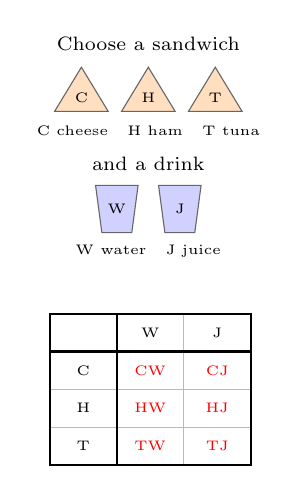
\begin{tikzpicture}[every node/.style={font=\tiny}]

% ---- The lunch deal: one sandwich and one drink ----
\node[font=\scriptsize] at (1.35,2.85) {Choose a sandwich};
\sarnie{0.5}{2.25}{C}
\sarnie{1.35}{2.25}{H}
\sarnie{2.2}{2.25}{T}
\node at (1.35,1.75) {C cheese \ \ H ham \ \ T tuna};
\node[font=\scriptsize] at (1.35,1.32) {and a drink};
\drink{0.95}{0.75}{W}
\drink{1.75}{0.75}{J}
\node at (1.35,0.22) {W water \ \ J juice};

% ---- The table every deal is listed in ----
\begin{scope}[yshift=-2.5cm, xshift=0.1cm]
\foreach \k in {0,1,2,3} \draw[gray!55] ({\k*0.85},0) -- ({\k*0.85},1.92);
\foreach \k in {0,1,2,3,4} \draw[gray!55] (0,{\k*0.48}) -- (2.55,{\k*0.48});
\draw[thick] (0,0) rectangle (2.55,1.92);
\draw[thick] (0.85,0) -- (0.85,1.92);
\draw[thick] (0,1.44) -- (2.55,1.44);
\node at (1.275,1.68) {W};
\node at (2.125,1.68) {J};
\node at (0.425,1.20) {C};
\node at (0.425,0.72) {H};
\node at (0.425,0.24) {T};
% the answers to question 4, written into the table
\node[anslab] at (1.275,1.20) {CW};
\node[anslab] at (2.125,1.20) {CJ};
\node[anslab] at (1.275,0.72) {HW};
\node[anslab] at (2.125,0.72) {HJ};
\node[anslab] at (1.275,0.24) {TW};
\node[anslab] at (2.125,0.24) {TJ};
\end{scope}

\end{tikzpicture}
\end{center}

\column{0.68\textwidth}
\vspace{-1.8em}
\footnotesize
\begin{ealglossed}
\begin{enumerate}\tightlist
\begin{multicols}{2}
  \item Write $\dfrac{2}{5}$ as a \ealgloss{decimal}{ułamek dziesiętny} and as a \ealgloss{percentage}{procent}.
        \ashow{$0.4=40\%$}
  \columnbreak
  \item Write $65\%$ as a \ealgloss{fraction}{ułamek} in its \ealgloss{simplest form}{najprostsza postać}.
        \ashow{$\tfrac{65}{100}=\tfrac{13}{20}$}
\end{multicols}
\begin{multicols}{2}
  \item A spinner lands on red, blue or green only. $P(\text{red})=0.35$,
        $P(\text{blue})=0.4$. Write $P(\text{green})$.
        \ashow{$1-0.35-0.4=0.25$}
  \columnbreak
  \item Complete the table to list every lunch deal.
\end{multicols}
\begin{multicols}{2}
  \item How many different lunch deals are there?
        \ashow{$6$}
  \columnbreak
  \item A deal is chosen at \ealgloss{random}{losowo}. Write $P(\text{juice})$ in its \ealgloss{simplest form}{najprostsza postać}.
        \ashow{$\tfrac{3}{6}=\tfrac{1}{2}$}
\end{multicols}
\begin{multicols}{2}
  \item Write $P(\text{cheese with water})$.
        \ashow{$\tfrac{1}{6}$}
  \columnbreak
  \item A third drink is added. How many deals are there now?
        \ashow{$3\times3=9$}
\end{multicols}
  \item Two \ealgloss{fair}{uczciwe} coins are flipped. List all the \ealgloss{outcomes}{wyniki} systematically, then write
        $P(\text{one head and one tail})$.
        \ashow{HH, HT, TH, TT, so $\tfrac{2}{4}=\tfrac{1}{2}$}
\end{enumerate}
\end{ealglossed}
\end{columns}
\end{frame}

%------------------------------------------------------------------
% STARTER 5: A sample space of two dice
%------------------------------------------------------------------
\begin{frame}[t,allowframebreaks]{Starter}
\begin{columns}[T]

\column{0.36\textwidth}
\vspace{-1.2em}
\begin{ealglossed}
{\scriptsize\raggedright Two \ealgloss{fair}{uczciwe}, ordinary dice are rolled, and the two numbers on them
are added together.\par}
\end{ealglossed}
\vspace{0.4em}
\begin{center}
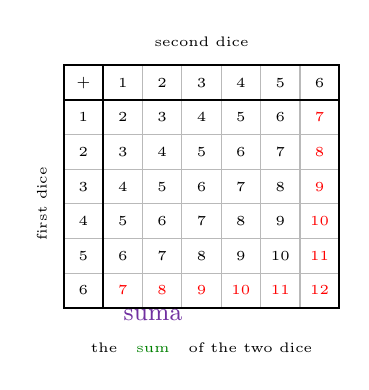
\begin{tikzpicture}[every node/.style={font=\tiny}]

% ---- The sums of two ordinary dice. The last row and the last column are the
% ---- answers to question 3, so the table is completed on the second overlay.
\foreach \k in {0,...,7} \draw[gray!55] ({\k*0.5},0) -- ({\k*0.5},3.08);
\foreach \k in {0,...,7} \draw[gray!55] (0,{\k*0.44}) -- (3.5,{\k*0.44});
\draw[thick] (0,0) rectangle (3.5,3.08);
\draw[thick] (0.5,0) -- (0.5,3.08);
\draw[thick] (0,2.64) -- (3.5,2.64);
\node at (0.25,2.86) {$+$};
\foreach \i in {1,...,6}{
  \node at (0.25,{2.86-0.44*\i}) {\i};
  \node at ({0.25+0.5*\i},2.86) {\i};
  \foreach \j in {1,...,6}{
    \pgfmathtruncatemacro{\s}{\i+\j}
    \ifnum\i<6
      \ifnum\j<6
        \node at ({0.25+0.5*\j},{2.86-0.44*\i}) {\s};
      \else
        \node[anslab] at ({0.25+0.5*\j},{2.86-0.44*\i}) {\s};
      \fi
    \else
      \node[anslab] at ({0.25+0.5*\j},{2.86-0.44*\i}) {\s};
    \fi
  }
}
\node at (1.75,-0.3) {the \ealgloss{sum}{suma} of the two dice};
\node[rotate=90, font=\tiny] at (-0.28,1.32) {first dice};
\node at (1.75,3.38) {second dice};

\end{tikzpicture}
\end{center}

\column{0.64\textwidth}
\vspace{-1.8em}
\footnotesize
\begin{ealglossed}
\begin{enumerate}\tightlist
\begin{multicols}{2}
  \item Write $\dfrac{1}{3}$ as a \ealgloss{decimal}{ułamek dziesiętny} and as a \ealgloss{percentage}{procent}.
        \ashow{$0.\dot{3}=33.\dot{3}\%$}
  \columnbreak
  \item Write $0.36$ as a \ealgloss{fraction}{ułamek} in its \ealgloss{simplest form}{najprostsza postać}.
        \ashow{$\tfrac{36}{100}=\tfrac{9}{25}$}
\end{multicols}
\begin{multicols}{2}
  \item Write the missing \ealgloss{sums}{sumy} in the table.
  \columnbreak
  \item How many \ealgloss{outcomes}{wyniki} are there altogether?
        \ashow{$6\times6=36$}
\end{multicols}
\begin{multicols}{2}
  \item Write $P(\text{the sum is }7)$ in its \ealgloss{simplest form}{najprostsza postać}.
        \ashow{$\tfrac{6}{36}=\tfrac{1}{6}$}
  \columnbreak
  \item Write the \ealgloss{probability}{prawdopodobieństwo} that the \ealgloss{sum}{suma} is more than $10$, in its \ealgloss{simplest form}{najprostsza postać}.
        \ashow{$\tfrac{3}{36}=\tfrac{1}{12}$}
\end{multicols}
  \item Which \ealgloss{sum}{suma} is the most \ealgloss{likely}{prawdopodobne}? Use its \ealgloss{probability}{prawdopodobieństwo} as a \ealgloss{percentage}{procent} to decide
        whether that \ealgloss{sum}{suma} is \ealgloss{likely}{prawdopodobne} or \ealgloss{unlikely}{mało prawdopodobne}.
        \ashow{$7$ is the most \ealgloss{likely}{prawdopodobne} \ealgloss{sum}{suma}, but $\tfrac{1}{6}=16.\dot{6}\%$, which is below $50\%$, so a \ealgloss{sum}{suma} of $7$ is still \ealgloss{unlikely}{mało prawdopodobne}.}
  \item The two dice are rolled $180$ times. How many times would you \ealgloss{expect}{oczekiwać} a \ealgloss{sum}{suma}
        of $5$?
        \ashow{$\tfrac{4}{36}=\tfrac{1}{9}$, and $\tfrac{1}{9}\times180=20$ times}
\end{enumerate}
\end{ealglossed}
\end{columns}
\end{frame}

%------------------------------------------------------------------
% STARTER 6: Completing a frequency tree
%------------------------------------------------------------------
\begin{frame}[t,allowframebreaks]{Starter}
\begin{columns}[T]

\column{0.38\textwidth}
\vspace{-1.2em}
\begin{ealglossed}
{\scriptsize\raggedright $80$ pupils sat a test. $50$ of them revised. Of the pupils who
revised, $44$ passed. Of the pupils who did not revise, $12$ passed. One of the $80$ pupils
is then chosen at \ealgloss{random}{losowo}.\par}
\end{ealglossed}
\vspace{0.4em}
\begin{center}
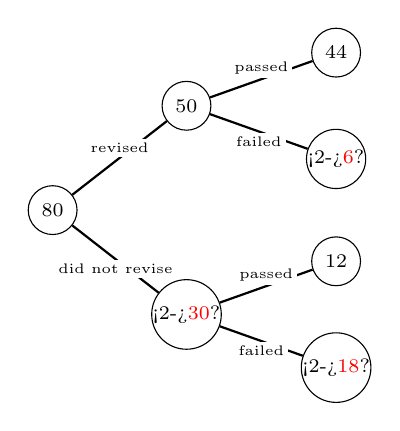
\begin{tikzpicture}

\node[ftnode] (t)  at (0,0)       {$80$};
\node[ftnode] (r)  at (1.7,1.325) {$50$};
\node[ftnode] (n)  at (1.7,-1.325){\dgap{$30$}};
\node[ftnode] (rp) at (3.6,2.0)   {$44$};
\node[ftnode] (rf) at (3.6,0.65)  {\dgap{$6$}};
\node[ftnode] (np) at (3.6,-0.65) {$12$};
\node[ftnode] (nf) at (3.6,-2.0)  {\dgap{$18$}};

\draw[ftarrow] (t) -- node[ftlab, above] {revised} (r);
\draw[ftarrow] (t) -- node[ftlab, below] {did not revise} (n);
\draw[ftarrow] (r) -- node[ftlab, above] {passed} (rp);
\draw[ftarrow] (r) -- node[ftlab, below] {failed} (rf);
\draw[ftarrow] (n) -- node[ftlab, above] {passed} (np);
\draw[ftarrow] (n) -- node[ftlab, below] {failed} (nf);

\end{tikzpicture}
\end{center}

\column{0.62\textwidth}
\vspace{-1.8em}
\footnotesize
\begin{ealglossed}
\begin{enumerate}\tightlist
\begin{multicols}{2}
  \item Write $\dfrac{3}{8}$ as a \ealgloss{decimal}{ułamek dziesiętny} and as a \ealgloss{percentage}{procent}.
        \ashow{$0.375=37.5\%$}
  \columnbreak
  \item A bag holds $9$ red and $1$ blue counter. Is taking a red counter \ealgloss{likely}{prawdopodobne}? Give
        $P(\text{red})$ as a \ealgloss{percentage}{procent}.
        \ashow{$\tfrac{9}{10}=90\%$, so \ealgloss{likely}{prawdopodobne}.}
\end{multicols}
\begin{multicols}{2}
  \item Complete the \ealgloss{frequency tree}{drzewko częstości}.
  \columnbreak
  \item How many pupils passed the test altogether?
        \ashow{$44+12=56$}
\end{multicols}
\begin{multicols}{2}
  \item Write $P(\text{revised})$ in its \ealgloss{simplest form}{najprostsza postać}.
        \ashow{$\tfrac{50}{80}=\tfrac{5}{8}$}
  \columnbreak
  \item Write $P(\text{revised and failed})$ in its \ealgloss{simplest form}{najprostsza postać}.
        \ashow{$\tfrac{6}{80}=\tfrac{3}{40}$}
\end{multicols}
  \item Write $P(\text{passed})$ as a \ealgloss{fraction}{ułamek}, a \ealgloss{decimal}{ułamek dziesiętny} and a \ealgloss{percentage}{procent}.
        \ashow{$\tfrac{56}{80}=\tfrac{7}{10}=0.7=70\%$}
  \item Is a pupil who revised more \ealgloss{likely}{prawdopodobne} to pass than a pupil who did not revise? Use
        \ealgloss{probabilities}{prawdopodobieństwa} to explain your answer.
        \ashow{Yes: $\tfrac{44}{50}=88\%$ of those who revised passed, against $\tfrac{12}{30}=40\%$ of those who did not.}
\end{enumerate}
\end{ealglossed}
\end{columns}
\end{frame}

%------------------------------------------------------------------
% STARTER 7: Working backwards through a frequency tree
%------------------------------------------------------------------
\begin{frame}[t,allowframebreaks]{Starter}
\begin{columns}[T]

\column{0.40\textwidth}
\vspace{-1.2em}
{\scriptsize\raggedright $200$ people took a driving test. $120$ of them were taking it
for the first time, and $84$ of those passed. Altogether $130$ people passed.\par}
\vspace{0.4em}
\begin{center}
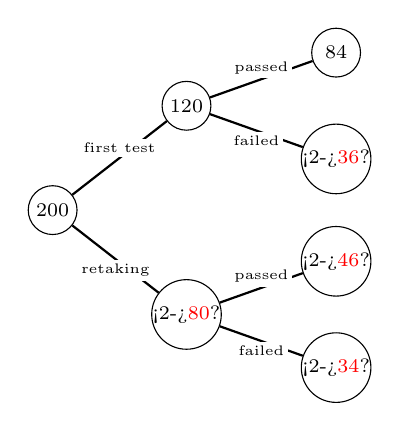
\begin{tikzpicture}

\node[ftnode] (t)  at (0,0)       {$200$};
\node[ftnode] (f)  at (1.7,1.325) {$120$};
\node[ftnode] (r)  at (1.7,-1.325){\dgap{$80$}};
\node[ftnode] (fp) at (3.6,2.0)   {$84$};
\node[ftnode] (ff) at (3.6,0.65)  {\dgap{$36$}};
\node[ftnode] (rp) at (3.6,-0.65) {\dgap{$46$}};
\node[ftnode] (rf) at (3.6,-2.0)  {\dgap{$34$}};

\draw[ftarrow] (t) -- node[ftlab, above] {first test} (f);
\draw[ftarrow] (t) -- node[ftlab, below] {retaking} (r);
\draw[ftarrow] (f) -- node[ftlab, above] {passed} (fp);
\draw[ftarrow] (f) -- node[ftlab, below] {failed} (ff);
\draw[ftarrow] (r) -- node[ftlab, above] {passed} (rp);
\draw[ftarrow] (r) -- node[ftlab, below] {failed} (rf);

\end{tikzpicture}
\end{center}

\column{0.60\textwidth}
\vspace{-1.8em}
\footnotesize
\begin{ealglossed}
\begin{enumerate}\tightlist
\begin{multicols}{2}
  \item Write $0.65$ as a \ealgloss{fraction}{ułamek} in its \ealgloss{simplest form}{najprostsza postać}.
        \ashow{$\tfrac{65}{100}=\tfrac{13}{20}$}
  \columnbreak
  \item Write $\dfrac{7}{8}$ as a \ealgloss{percentage}{procent}.
        \ashow{$87.5\%$}
\end{multicols}
\begin{multicols}{2}
  \item A bag holds $7$ green and $3$ red counters. Write $P(\text{green})$ as a
        \ealgloss{percentage}{procent}.
        \ashow{$\tfrac{7}{10}=70\%$}
  \columnbreak
  \item Complete the \ealgloss{frequency tree}{drzewko częstości}.
\end{multicols}
\begin{multicols}{2}
  \item Write $P(\text{passed})$ in its \ealgloss{simplest form}{najprostsza postać} and as a \ealgloss{percentage}{procent}.
        \ashow{$\tfrac{130}{200}=\tfrac{13}{20}=65\%$}
  \columnbreak
  \item Write the \ealgloss{probability}{prawdopodobieństwo} that a person took the test for the first time and passed.
        \ashow{$\tfrac{84}{200}=\tfrac{21}{50}$}
\end{multicols}
  \item What \ealgloss{percentage}{procent} passed on a first test, and what \ealgloss{percentage}{procent} passed on a retake?
        \ashow{$\tfrac{84}{120}=70\%$ and $\tfrac{46}{80}=57.5\%$}
  \item Jo says ``people are more \ealgloss{likely}{prawdopodobne} to pass a retake, because they have had more
        practice''. Do these figures support Jo?
        \ashow{No: $70\%$ passed on a first test, but only $57.5\%$ on a retake.}
\end{enumerate}
\end{ealglossed}
\end{columns}
\end{frame}

%------------------------------------------------------------------
% STARTER 8: Probabilities from a Venn diagram
%------------------------------------------------------------------
\begin{frame}[t,allowframebreaks]{Starter}
\begin{columns}[T]

\column{0.42\textwidth}
\vspace{-1.2em}
\begin{ealglossed}
{\scriptsize\raggedright $40$ pupils were asked which sports they play. $24$ play
football, $16$ play cricket, and $8$ play both. One pupil is then chosen at \ealgloss{random}{losowo}.\par}
\end{ealglossed}
\vspace{0.5em}
\begin{center}
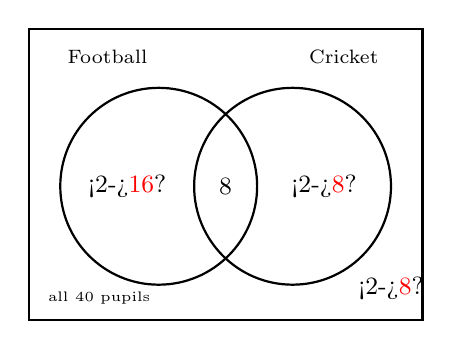
\begin{tikzpicture}[every node/.style={font=\scriptsize}]

\draw[vset] (0,0) rectangle (5.0,3.7);
\draw[vset] (1.65,1.7) circle (1.25);
\draw[vset] (3.35,1.7) circle (1.25);
\node at (1.0,3.35) {Football};
\node at (4.0,3.35) {Cricket};
\node[font=\tiny, anchor=west] at (0.12,0.28) {all $40$ pupils};

% the answers to question 3, written into the regions of the diagram
\node[vnum] at (1.25,1.7) {\dgap{$16$}};
\node[vnum] at (2.5,1.7)  {$8$};
\node[vnum] at (3.75,1.7) {\dgap{$8$}};
\node[vnum] at (4.6,0.4)  {\dgap{$8$}};

\end{tikzpicture}
\end{center}

\column{0.58\textwidth}
\vspace{-1.8em}
\footnotesize
\begin{ealglossed}
\begin{enumerate}\tightlist
\begin{multicols}{2}
  \item Write $0.2$ as a \ealgloss{fraction}{ułamek} in its \ealgloss{simplest form}{najprostsza postać} and as a \ealgloss{percentage}{procent}.
        \ashow{$\tfrac{1}{5}=20\%$}
  \columnbreak
  \item A caf\'e sells $4$ sandwiches and $3$ drinks. How many deals of one sandwich
        and one drink are there?
        \ashow{$4\times3=12$}
\end{multicols}
\begin{multicols}{2}
  \item How many pupils play football but not cricket?
        \ashow{$24-8=16$}
  \columnbreak
  \item Complete the \ealgloss{Venn diagram}{diagram Venna}.
\end{multicols}
\begin{multicols}{2}
  \item Write $P(\text{cricket})$ in its \ealgloss{simplest form}{najprostsza postać} and as a \ealgloss{percentage}{procent}.
        \ashow{$\tfrac{16}{40}=\tfrac{2}{5}=40\%$}
  \columnbreak
  \item Write $P(\text{neither sport})$ in its \ealgloss{simplest form}{najprostsza postać}.
        \ashow{$\tfrac{8}{40}=\tfrac{1}{5}$}
\end{multicols}
  \item Write $P(\text{football or cricket})$ in its \ealgloss{simplest form}{najprostsza postać} and as a \ealgloss{percentage}{procent}.
        \ashow{$\tfrac{32}{40}=\tfrac{4}{5}=80\%$}
  \item $P(\text{football})+P(\text{cricket})=\tfrac{3}{5}+\tfrac{2}{5}=1$, but
        $P(\text{football or cricket})=\tfrac{4}{5}$. Explain why these are different.
        \ashow{The $8$ who play both are in both circles, so they are counted twice.}
\end{enumerate}
\end{ealglossed}
\end{columns}
\end{frame}

%------------------------------------------------------------------
% STARTER 9: Sorting into a Venn diagram, then reading probabilities off it
%------------------------------------------------------------------
\begin{frame}[t,allowframebreaks]{Starter}
\begin{columns}[T]

\column{0.42\textwidth}
\vspace{-1.2em}
\begin{ealglossed}
{\scriptsize\raggedright One of the numbers from $1$ to $20$ is chosen at \ealgloss{random}{losowo}.\par}
\end{ealglossed}
\vspace{0.4em}
\begin{center}
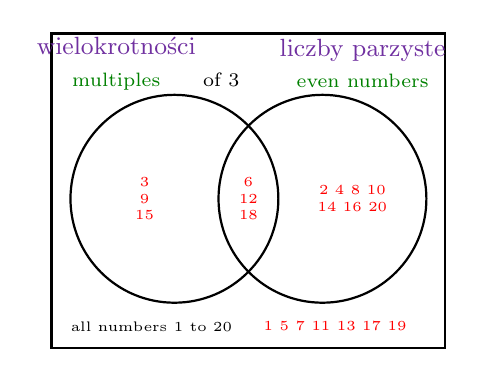
\begin{tikzpicture}[every node/.style={font=\scriptsize}]

\draw[vset] (0,0) rectangle (5.0,4.0);
\draw[vset] (1.56,1.9) circle (1.32);
\draw[vset] (3.44,1.9) circle (1.32);
\node at (1.10,3.62) {\ealgloss{multiples}{wielokrotności} of $3$};
\node at (3.95,3.62) {\ealgloss{even numbers}{liczby parzyste}};
\node[font=\tiny, anchor=west] at (0.12,0.28) {all numbers $1$ to $20$};

% the answers to question 3, written into the regions of the diagram
\node[anslab, align=center] at (1.18,1.9) {$3$\\$9$\\$15$};
\node[anslab, align=center] at (2.50,1.9) {$6$\\$12$\\$18$};
\node[anslab, align=center] at (3.82,1.9) {$2$\ $4$\ $8$\ $10$\\$14$\ $16$\ $20$};
\node[anslab] at (3.60,0.28) {$1$\ $5$\ $7$\ $11$\ $13$\ $17$\ $19$};

\end{tikzpicture}
\end{center}

\column{0.58\textwidth}
\vspace{-1.8em}
\footnotesize
\begin{ealglossed}
\begin{enumerate}\tightlist
\begin{multicols}{2}
  \item Write $\dfrac{3}{20}$ as a \ealgloss{decimal}{ułamek dziesiętny} and as a \ealgloss{percentage}{procent}.
        \ashow{$0.15=15\%$}
  \columnbreak
  \item Write $35\%$ as a \ealgloss{fraction}{ułamek} in its \ealgloss{simplest form}{najprostsza postać}.
        \ashow{$\tfrac{35}{100}=\tfrac{7}{20}$}
\end{multicols}
\begin{multicols}{2}
  \item Write each number from $1$ to $20$ in the correct region.
  \columnbreak
  \item A number goes in the \ealgloss{overlap}{część wspólna} when it is a \ealgloss{multiple}{wielokrotność} of \ablank{$\;6\;$}.
\end{multicols}
\begin{multicols}{2}
  \item Write $P(\text{multiple of }3)$ in its \ealgloss{simplest form}{najprostsza postać}.
        \ashow{$\tfrac{6}{20}=\tfrac{3}{10}$}
  \columnbreak
  \item Write the \ealgloss{probability}{prawdopodobieństwo} that the number is neither even nor a \ealgloss{multiple}{wielokrotność} of $3$.
        \ashow{$\tfrac{7}{20}$}
\end{multicols}
  \item Is the number \ealgloss{likely}{prawdopodobne} or \ealgloss{unlikely}{mało prawdopodobne} to be a \ealgloss{multiple}{wielokrotność} of $3$? Use its \ealgloss{probability}{prawdopodobieństwo} as
        a \ealgloss{percentage}{procent} to explain.
        \ashow{$\tfrac{3}{10}=30\%$, which is below $50\%$, so \ealgloss{unlikely}{mało prawdopodobne}.}
  \item Choose two new labels for the circles so that the \ealgloss{overlap}{część wspólna} must be empty, and
        explain why.
        \ashow{For example ``odd'' and ``even'': no number is both odd and even.}
\end{enumerate}
\end{ealglossed}
\end{columns}
\end{frame}

\end{document}